\chapter{Part I: Column Store}
\label{chap:column-store}

In this chapter, we modify how \gap~represents data internally by replacing the original row storage format with a column store. We see how it successfully reduces memory consumption and load times for the \tpch.

This chapter makes up the first out of four main iterations in the design and experiment part of this research. As mentioned in the introduction, we aim to reduce memory consumption in the first iterations of the research.

\clearpage

\section{Introduction}
\label{sec:Introduction}
% Tell how we want to reduce memory and how database technology comes to the rescue
In the first part of this thesis, we aim to reduce memory footprint such that memory client memory requirements can be relaxed. As we saw in Section \ref{sec:Compression}, lower memory usage are likely to increase performance because most database processes are memory-bound. Moreover, we hypothesize that memory management is expensive and that the number of allocations, as well as the size of the allocated memory chunks, should be reduced. Inspired by the techniques used by read-optimized databases in Chapter \ref{chap:olap} and motivated by the challenges in \gap, we change how data is represented internally in the platform.

% tell why we picked a column store
We choose to implement a column store, which we read about in Section \ref{sec:Column Storage}. The reason for this is two-fold. First, as we saw in the literature study, columns are inherently more compressible. Hence, a column store is better suited to reduce memory consumption and to test our hypothesis about the costs of memory management. Second, the cases where \genus~has experienced performance issues are in situations where a column store is better suited than a row store, for instance on join and filter operations.

% Tell why we did not pick a row store
We believe that conventional transactional processing in \gap, where a row store might be better suited, will not suffer from using a column store. There is much overhead on create, update, and delete operations, like constraint checks, data validation, and memory allocations that will make the column store overhead negligible. Also, a row store might require index structures to accommodate certain operations; indexes which, as we have seen in Section \ref{sub:Row Stores vs Column Stores}, are costly to maintain.

\section{Implementation}
\label{sec:Implementation}
\todo{Go over entire Implementation section}

In this section, we explain how a column store is implemented in \gap~by introducing data source indexes and replacing \cn{CompositionObjectValueCollection}.

\subsection{CompositionValueCollection}
\label{sub:CompositionValueCollection}
% Lineout the challenges
As we saw in Section \ref{sec:Challenges in Genus App Platform}, one of the challenges in \gap~is the \cn{CompositionObjectValueCollection} class that not only holds the data belonging to each object, but also pointers to the data descriptors. Although this class is flexible because it is self-contained, and can be passed among objects to copy values, for most cases, references to the data descriptors does not need to be stored per data collection. 

% Conceptually what is done
\begin{figure}
    \centering
    \begin{subfigure}{1.0\textwidth}
        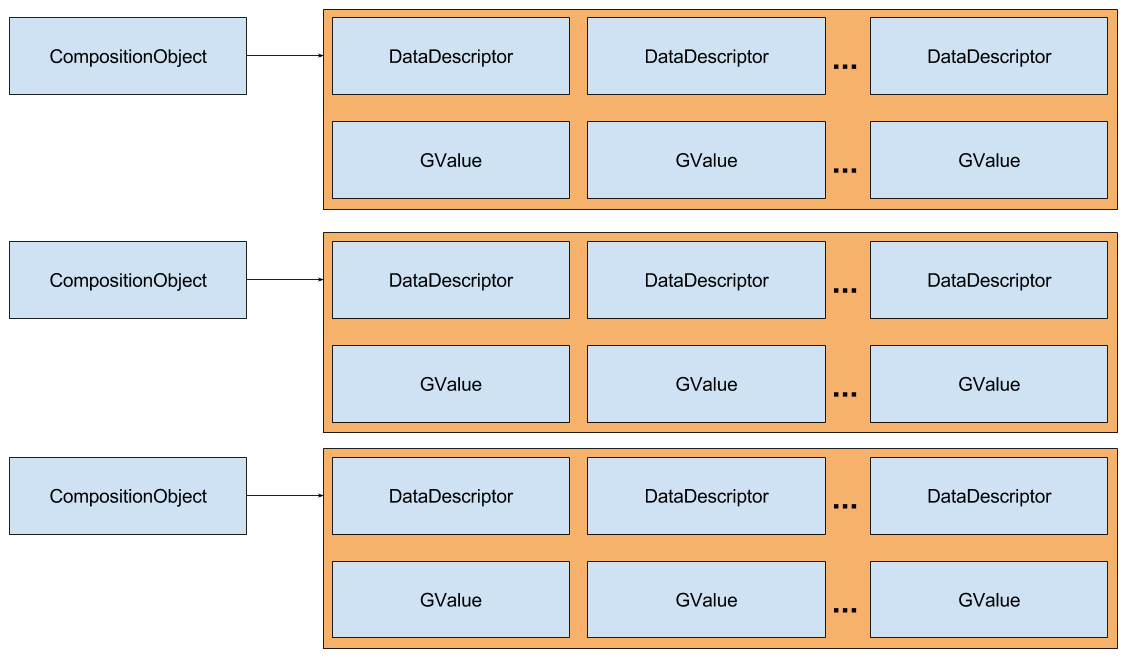
\includegraphics[width=\textwidth]{img/gap-original-rows.png}
        \caption{Original implementation with \cn{CompositionObjectValueColletion}. Each object has its own value collection structure, and each value collection contains pointers to the data descriptors and to the data.}
        \label{fig:gap-original-rows}
    \end{subfigure}
    \begin{subfigure}{1.0\textwidth}
        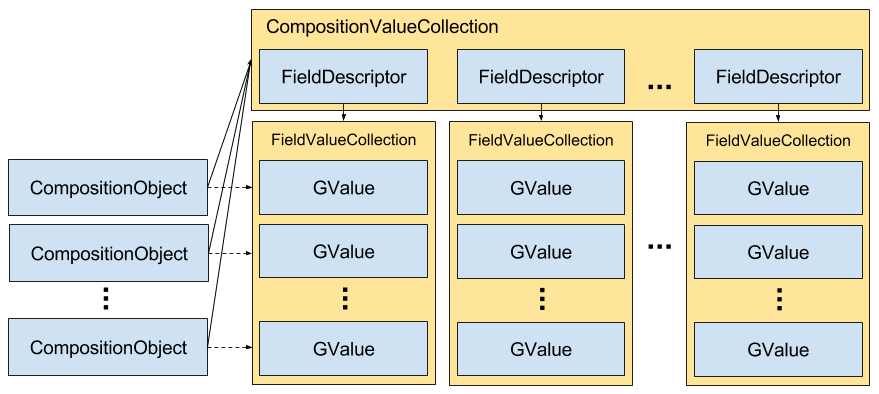
\includegraphics[width=\textwidth]{img/gap-bb-columns.png}
        \caption{Column store implementation with \cn{CompositionValueColletion} and \cn{FieldValueCollection}. All objects in a data source point to the same value collection, and access data using its datasource index, or row identifier, that indicates which column index holds the data.}
        \label{fig:gap-bb-columns}
    \end{subfigure}
    \caption{Comparison of the original implementation and the column store implementation.}
    \label{fig:gap-storage-comparison}
\end{figure}
In our column store, we plan to replace the \cn{CompositionObjectValueCollection} pointer in each \cn{CompositionObject} with a pointer to a \cn{CompositionValueCollection} and an integer, \cn{DatasourceIndex}, that indicates which position in the data source the object has. The data source variable can be thought of as a row identifier, which we studied in Section \ref{sub:Row Identifiers and Tuple Materialization}. All objects within a data source has a pointer to the same \cn{CompositionValueCollection}. This means that composition objects no longer will query its own data collection for values, but rather one common data collection used by all objects. To access a certain value, both \cn{DataDescriptor} and \cn{DatasourceIndex} is required to indicate column and row respectively. A comparison of the old and the new implementation is seen in \ref{fig:gap-storage-comparison}.

\todo{section on tuple materialization?}

% How it impacts memory
In Section \ref{sub:Excessive Amount Of Pointers}, we saw how a data source with objects with 15 properties each needed 32 pointers, or 256 bytes, per objects just for data and data access. Now, this number is reduced to 17 pointers and an integer, which is 140 bytes. Hence, we have the potential to save 45\% memory by using our new system.

% CompositionObjectValueCollection still exists
Even though the original \cn{CompositionObjectValueCollection} was discarded as the main storage structure, composition objects can still assemble such structures by querying the \cn{CompositionValueCollection}. This is used in object cloning and to transfer data across different data sources in different parts of the application \todo{Stemmer dette?}.

% class diagram
% explain the dictionary and the list of data descriptors
\afigure{img/CompositionValueCollection.png}{\cn{CompositionValueCollection} class diagram.}{fig:CompositionValueCollection}{0.9}
The \cn{CompositionValueCollection} is a class type. The class diagram is shown in Figure \ref{fig:CompositionValueCollection}.

The main methods in the \cn{CompositionValueCollection} class is the \fn{setValue} and \fn{getValue} methods. These functions respectivel set and get \cn{GValues} for a data descriptor and a datasource index. In these operations, the correct column, or \cn{FieldValueCollection}, is looked up in a dictionary, and the index is passed along to the column to get or set the value. If no column exist for a data descriptor, it is created. \fn{isAssigned} and \fn{unassignValue} works similarly. We study the unassigned semantic in Section \ref{sub:Unassigned Values}. 

Datasource indexes are assigned by passing composition objects to the  \fn{registerObject} function. A private variable \vn{maxDatasourceIndex} is used to keep track on the maximum index handed out so far. When an object is received, this variable is incremented, and the object is assigned that value. In addition to this, a bitmap \fn{assignedIndexes} is kept to bookkeep which indexes has objects connected to them. When \fn{removeObject} is called, the bit for that index is unset in \fn{assignedIndexes}. Also, all values corresponding to that object are unassigned. Currently, the \fn{assignedIndexes} bitmap is not used to lookup the first available bit, since this triggers a linear search on every insertion. We discuss this further in the chapter conclusion.

In addition to the above methods, a \cn{CompositionValueCollection} has the ability to unassign an entire row or column by passing in a \cn{CompositionObject} or \cn{DataDescriptor} respectively. We see later in this research where such methods are used.

The \fn{Consolidate} function is called by the data source when it is done loading and is meant to be an operation where the column store restructures and maximizes space utilization. We see how the columns are affected by this operation in the section about growth strategy, Section \ref{sec:Growth Strategy}.


\subsection{FieldValueCollection}
\label{sub:FieldValueCollection}
\afigure{img/FieldValueCollection.png}{\cn{FieldValueCollection} class diagram.}{fig:FieldValueCollection}{0.55}

A column is implemented as a \cn{FieldValueCollection} class, and is an index based list structure that automatically handles reallocation. \cn{GValue}s are stored in a \cn{TArray<GValue>}. This array structure was picked based on the performance benchmark in Appndix \ref{app:array-types}. A class diagram for the \cn{FieldValueCollection} is found in Figure \ref{fig:FieldValueCollection}.

Setting a value to \vn{null} has different semantics than \fn{UnassignValue}. The latter means that there has previously been a value present, but is now removed for performance reasons. This functionality is implemented using a bitmap, \cn{BasicBitArray}, which is based on \delphi~\cn{TBits} type. \todo{Stemmer dette om Unassigned values?}

\subsection{Growth Strategy}
\label{sub:Growth Strategy}
Since we used native dynamic arrays, we control the array allocation size. For every reallocation, we risk that the entire array needs to be copied from one part of the memory to another. For this reason, one should be generous when allocating, ideally, allocate the correct size immediately. However, since we read a stream of data objects, we are not sure how large our buffers should until the very end. 

\afigure{img/gap-growth-strategy.png}{Growth strategy for buffers. In the load phase, the buffer doubles every time more space is needed. After the load phase, a consolidation is performed which reduces the buffer size to the exact number which is contained in a column.}{fig:gap-growth-strategy}{0.6}
Therefore, we chose a strategy where we double the buffer size every time we need more space. This way, the number of reallocation operations are kept to a minimum. However, this strategy might result in lots of unused buffer space. We, therefore, add a \fn{Consolidate} function to our column store that resizes all buffers to fit its data. The strategy is depicted in \ref{gap-growth-strategy}.

\subsection{Modifying CompositionObject}
\label{sub:Modifying CompositionObject}
% Change value collections and add index
In order for the \cn{CompositionObject} class, some some adjustments are made. First and foremost, the \cn{CompositionObjectValueCollection} are replaced with a \cn{CompositionValueCollection} class. All code that accesses the original structure are rewritten to use the column store, where the data source index is passed as a parameter. The \cn{CompositionValueCollection} is already created by the data source, and is sent in as a parameter in the constructor. It must no longer ask its value collection; it must send itself and its data source index into the GetValue. It no longer holds ownership to a collection but has a pointer to a value collection shared by all composition objects.

% Constructor and destructor calls
Second, \fn{RegisterObject} is called within the constructor such that the \cn{CompositionObject} get a datasource index. Analogously, \fn{RemoveObject} is called in the destructor.

% Adapt to the existing value collections with adapts and clone
The class is extended by creating a \fn{CloneValueCollection} that creates a row in the original format. Similarly, a method \fn{AdoptValueCollection} is set up to fill in data from a row structure.

\section{Results}
\label{sec:Results}
We test the changes done in this iteration by using Benchmark \ref{bm:q1}, the \textit{TPC-H Q1 Data Load Benchmark}. We use this benchmark to see whether memory footprint has been reduced. We are also curious to see the performance impact on data load time, lookup index generation (join), and source measure lookup. To see whether our changes has caused negative effects on write performance, we also run Benchmark \ref{bm:write}, the \textit{Write Benchmark}. 

Full benchmark details are found in Appendix \ref{app:bm}.

\subsection{TPC-H Q1 Data Load Benchmark}
\label{column-store:q1}
Benchmark \ref{bm:q1}, \textit{TPC-H Q1 Data Load Benchmark}, was run with the original and the new column-store implementation with scaling factors 0.01 and 0.1. Each configuration was run three times, and the average of the runs is reported. Only three tests were run due to time constraints. However, all results were within 15 \% of the average value.

\begin{table}
    \centering
    \begin{tabularx}{0.75\textwidth}{X | X X}
        & SF0.01 & SF0.1 \\ 
        \hline
        \hline
        Original & 674 bytes & 715 bytes \\
        Column Store & 419 bytes & 501 bytes \\
        \% reduction & 38 \% & 30 \% \\
    \end{tabularx}
    \caption{Bytes per \texttt{LINEITEM} used by the original and the new column store implementation.} 
    \label{tab:non-blackbox-bpl}
\end{table}
We found a drastic memory reduction with the column store implementation. As seen in Table \ref{tab:non-blackbox-bpl}, the SF0.01 test reduces the memory per \texttt{LINEITEM} by 38 \%, and SF0.1 reduces it by 30 \%. For SF0.1, we also used the total memory footprint output. Total application memory consumption was reduced from 2685 MB to 1777 MB, which is a reduction of 34 \%.

\begin{table}
    \centering
    \begin{tabularx}{0.75\textwidth}{X | X X}
        & SF0.01 & SF0.1 \\ 
        \hline
        \hline
        Original & 2302 ms & 23164 ms \\
        Column Store & 842 ms & 8539 ms \\
        \% reduction & 63 \% & 63 \% \\
    \end{tabularx}
    \caption{Load times for Benchamrk \ref{bm:q1} for the original and the new column store implementation and scaling factors 0.01 and 0.1.} 
    \label{tab:non-blackbox-load}
\end{table}
We see that the load times also is drastically reduced using \cn{CompositionValueCollection}. For both scaling factors, the time it takes to load the datasource with object has been reduced by 63 \%. The results are presented in Table \ref{tab:non-blackbox-load}.

\begin{table}
    \centering
    \begin{tabularx}{0.9\textwidth}{X | X X X}
        SF0.01 & \texttt{LINESTATUS} & \texttt{RETURNFLAG} & \texttt{SHIPDATE}\\ 
        \hline
        \hline
        Original & 300 ms & 313 ms & 1385 ms \\
        Column Store & 391 ms & 401 ms & 1398 ms \\
    \end{tabularx}
    \newline
    \vspace*{1 cm}
    \newline
    \begin{tabularx}{0.9\textwidth}{X | X X X}
        SF0.1 & \texttt{LINESTATUS} & \texttt{RETURNFLAG} & \texttt{SHIPDATE}\\ 
        \hline
        \hline
        Original & 2939 ms & 2849 ms & 13144 ms \\
        Column Store & 3123 ms & 3301 ms & 13004 ms \\
    \end{tabularx}
    \caption{Lookup index generation performance comparison for \texttt{LINESTATUS}, \texttt{RETURNFLAG}, and \texttt{SHIPDATE} for SF0.01 (upper) and SF0.1 (lower).} 
    \label{tab:non-blackbox-lig}
\end{table}
As seen in Table \ref{tab:non-blackbox-lig}, the lookup index generation, or join operation, is hurt by the \cn{CompositionValueCollection} implementation. For scaling factor 0.01, the time it takes to join \texttt{LINESTATUS} and \texttt{RETURNFLAG} with the \texttt{LINEITEM} table is increased by approximately 30 \%.


\begin{table}
    \centering
    \begin{tabularx}{\textwidth}{X | X X X X}
        SF0.01 & \texttt{QUANTITY} & \texttt{EXTENDEDPRICE} & \texttt{DISCOUNT} & \texttt{TAX}\\ 
        \hline
        \hline
        Original & 30 ms & 34 ms & 32 ms & 35 ms \\
        Column Store & 57 ms & 67 ms & 75 ms & 76 ms
    \end{tabularx}
    \newline
    \vspace*{1 cm}
    \newline
    \begin{tabularx}{\textwidth}{X | X X X X}
        SF0.01 & \texttt{QUANTITY} & \texttt{EXTENDEDPRICE} & \texttt{DISCOUNT} & \texttt{TAX}\\ 
        \hline
        \hline
        Original & 302 ms & 385 ms & 312 ms & 369 ms \\
        Column Store & 532 ms & 625 ms & 646 ms & 752 ms
    \end{tabularx}
    \caption{Source measure lookup for \texttt{QUANTITY} \texttt{EXTENDEDPRICE}, \texttt{DISCOUNT}, and \texttt{TAX} for SF0.01 (upper) and SF0.1 (lower).} 
    \label{tab:non-blackbox-sml}
\end{table}
We also see that source measure looukup is also hurt by the new column store implementation, where the the time it takes to extract all values into a floating point array is doubled. The results are presented in Table \ref{tab:non-blackbox-sml}.

\subsection{Write Benchmark}
\label{sub:Write Benchmark}
To see how the write speed is affected by our new implementation, we run Benchmark \ref{bm:write}, the \textit{Write Benchmark} on the original implementation and the column store implementation. Each run modified 1000 elements. Due to time constraints, there were only three runs per implementation. However, most measurements were within 15 \% of the average.

\begin{table}
    \begin{tabularx}{\textwidth}{X | X X X X}
         & \texttt{QUANTITY} & \texttt{EXTENDEDPRICE} & \texttt{COMMENT} & \texttt{SHIPDATE}\\ 
        \hline
        \hline
        Original & 1657 ms & 1675 ms & 1669 ms & 2060 ms \\
        Column Store & 1642 ms & 1610 ms & 1770 ms & 2046 ms
    \end{tabularx}
    \caption{Test results for Benchmark \ref{bm:write}.}
    \label{tab:non-blackbox-write}
\end{table}
The results are presented in Table \ref{tab:non-blackbox-write}. There are not more differences between the two implementations that are expected by random, except for \texttt{COMMENT}. This result had an outlier.

\section{Discussion}
\label{sec:Discussion}
We see that the memory used per object in the \textit{TPC-H Q1 Data Load Benchmark} is reduced by 30 \% and 38 \% for scaling factors 0.1 and 0.01 respectively. We attribute the memory reduction to the column store, and how it reduces the number of pointers needed to represent data in a data source.

We are excited to observe that the data source load time is drastically reduced as a consequence of our new \cn{CompositionValueCollection} and \cn{FieldValueCollection} classes. This observation strengthens our hypothesis that memory management is expensive: The original implementation allocated one row-structure per object, whereas the doubling strategy in our column store keeps the number of allocations at a minimum. Moreover, the reduced load time in Benchmark \ref{bm:q1}~might also imply that reduced memory usage is directly correlated with performance and that our new implementation has better memory locality and cache hit rate.

Both read operations, lookup index generation and source measure lookup, suffer from the new column store implementation. On these operations, the time it takes to perform the operation has been increased by 30 \% and 100 \% respectively. Since both operations read values intensively from composition objects in tight loops, we believe the test result implies that the \fn{GetValue} function in the column store is not as efficient as the original. This can be caused by the dictionary lookup to find the correct column, or by the extra checks to ensure capacity or for \nil~values.

The fact that Benchmark \ref{bm:write}, the \textit{Write Benchmark}, shows that write performance is not affected by the column store, strengthens our hypothesis that the column overhead is negligible in such situations. Data modification is expensive in \gap. Modifying 1000 elements in the write benchmark takes roughly five times longer than generating a lookup index for 60,000 rows, which indicates that there is a severe overhead in object iteration and value modification unrelated to the data storage layout.

We are unsure why different scaling factors yielded a different number of bytes per \lineitem. It might be caused by the caching and value reuse mechanisms used by the data load module in \gap. Data in SF0.1 might have a different data distribution than SF0.01. Either way, both the original and column store implementations are affected by this phenomenon, which makes it likely that it is unrelated to our work.

\section{Iteration Conclusion}
\label{sec:Iteration Conclusion}
We conclude this iteration by stating that there is a large potential in column storage regarding memory footprint and load times. Memory used per \lineitem~in the \textit{TPC-H Q1 Data Load Benchmark} has been reduced by 30 - 38 \%, and the time it takes to load all data in this benchmark by 67 \%. Write performance, tested with Benchmark \ref{bm:write}, has not been affected by the new implementation.

Still, both read-intense operations tested in Benchmark \ref{bm:q1}, especially the source measure lookup operation. Here, the time it takes to generate an array of double precision numbers for a data descriptor is doubled with the column store. We believe this changes are caused by a \fn{GetValue} function less efficient than the original.

This iteration lays the groundwork for further investigation and to check whether database technologies and column store can help \mdd-tools' ability to handle and analyse large datasets. We believe even more memory can be saved by optimizing storage formats, applying compression, and removing more pointers. We do this in the next iterations, Chapter \ref{chap:storage-format} and Chapter \ref{chap:compression}. 

Column storage comes with several benefits, like vectorized execution, late materialization, and the ability to be pipelined by a modern CPU. We have not yet utilized the full potential of the \cn{CompositionValueCollection} and \cn{FieldValueCollection} classes, so far we have only used them to reduce the number of pointers in \gap. We believe the mentioned techniques can be applied to the read-intense operations of Benchmark \ref{bm:q1}. We study this in Chapter \ref{chap:operations}.

\subsection{Future Work}
\label{sub:Future Work}
With our current solution, new data source indexes, or row identifiers, are assigned by incrementing a counter in \cn{CompositionValueCollection}. This implies that if objects are removed from a data source, no new objects will be assigned the data source indexes that has become available. As seen in Figure \ref{fig:CompositionValueCollection}, we propose a \textit{bitmap for assigned indexes}, \vn{assignedFlags}. Future work might investigate the effects of using this bitmap, and the \fn{OpenBit} utility function, to assign indexes to a data source. Since \fn{OpenBit} is a linear-time operation, one might consider an object loading state: Indexes are assigned by using a counter if the data source is fed with data from the database, and once this operation has completed, the \vn{assignedFlags} bitmap is used.


%In addition, we have observed that the bytes per \texttt{LINEITEM} is increased on larger data sets, and we believe this is caused by the caching and value reuse mechanisms in the data source loader. However, larger datasets should be able to reuse more values, not less. We therefore encourage studying this peculiar effect in future work.
